\addtotoc{Summary (English)}
\thispagestyle{plain}

\vspace*{-6mm}
\begin{center}
\textbf{\large \titlenameEN}\\[1mm]
\end{center}

\begin{flushright}
\departmentnameEN\\
Student: \studentID, \authorShortEN\\
Supervisor: \supervisornameEN
\end{flushright}

\vspace{1mm}
\setcounter{table}{0}
\setcounter{figure}{0}
\renewcommand{\thetable}{\arabic{table}}
\renewcommand{\thefigure}{\arabic{figure}}
\setlength{\columnsep}{7mm}
\begin{multicols}{2}
\setlength{\parskip}{5pt}
\sloppy

\noindent\textbf{1. Introduction}

This research addresses the development of a fully automated 3D reconstruction pipeline and graphical user interface (GUI) from multi-view 2D images, as well as the experimental evaluation of how matching parameters affect reconstruction accuracy. Traditional Structure-from-Motion (SfM) and Multi-View Stereo (MVS) methods offer strong geometric precision but impose high computational demands, and parameter choices significantly affect output quality.

The research objectives were to: develop a 9-stage pipeline based on COLMAP and OpenMVS; build a PyQt5-based GUI system; experimentally evaluate the effect of matcher choice and matching strategy on accuracy; measure reconstruction quality using Chamfer Distance and RMSE; and transparently document the limitations of the study. Chamfer Distance and RMSE were used as evaluation metrics --- lower values indicate a closer match to the ground truth.

\noindent\textbf{2. Background and Related Work}

Key prior work includes: Hartley \& Zisserman (2003) on multi-view geometry foundations; Lowe's (2004) SIFT for scale- and rotation-invariant features; Sch{\"o}nberger \& Frahm's (2016) COLMAP incremental SfM pipeline; and Cernea's (2015) OpenMVS dense reconstruction toolkit. Modern methods such as NeRF (Mildenhall et al., 2020) and 3D Gaussian Splatting (Kerbl et al., 2023) excel in rendering quality but demand substantially more compute. This research adopted the classical COLMAP+OpenMVS approach for its reliability and flexibility for future ML integration.

\noindent\textbf{3. Methodology and Implementation}

The pipeline was implemented in Python (\texttt{core/}, \texttt{pipeline/}, \texttt{gui/}, \texttt{utils/} modules). The PyQt5 GUI provides a progress bar, real-time log output, and mid-run abort capability. Hardware: NVIDIA RTX 4060, Intel Core i9 (15th Gen), 16\,GB RAM.

Three separate datasets were used across the experiments (Table~\ref{tab:summary_en_datasets}). The Temple Ring and Caterpillar datasets consist of object photos captured at $1920\times1080$ JPEG resolution. Experiment 3 additionally used a publicly available 4K Lighthouse video (5:45, 23.98\,fps, $4096\times2160$) as an outdoor, real-world reconstruction test --- this footage was not captured by the authors.

\begin{table}[H]
\centering
\caption{Experimental datasets}
\label{tab:summary_en_datasets}
\scriptsize
\setlength{\tabcolsep}{3pt}
\begin{tabular}{|l|r|l|}
\hline
\textbf{Dataset} & \textbf{Images} & \textbf{Used in} \\ \hline
Temple Ring & 47 & Exp.\ 1 \\ \hline
Caterpillar & 380~ & Exp.\ 2 \\ \hline
Lighthouse 4K video & ${\sim}$86/172/200 frames & Exp.\ 3 \\ \hline
\end{tabular}
\end{table}

Three experiment series were conducted:
\begin{itemize}
    \item \textbf{Exp.\ 1:} SIFT vs.\ LightGlue $\times$ exhaustive vs.\ sequential (overlap=10), on Dataset A.
    \item \textbf{Exp.\ 2:} Sequential overlap values 5, 10, 20, 40 on Dataset A.
    \item \textbf{Exp.\ 3:} Frames from the Lighthouse video at 4\,s/2\,s/1.5\,s intervals (${\sim}86$, ${\sim}172$, ${\sim}200$ frames).
\end{itemize}

\noindent\textbf{4. Results and Conclusions}

Key system performance metrics:

\begin{table}[H]
\centering
\caption{Key system performance metrics (Dataset A)}
\label{tab:summary_en_results}
\scriptsize
\setlength{\tabcolsep}{3pt}
\begin{tabular}{|l|r|}
\hline
\textbf{Metric} & \textbf{Value} \\ \hline
Dataset A (images) & 47 \\ \hline
Sparse point cloud & 35{,}000+ points \\ \hline
Dense point cloud & 2.1 million points \\ \hline
Mesh vertices / faces & 1.2M / 2.3M \\ \hline
Best CD (1B: LG+Exhaustive) & 0.0074\,m \\ \hline
Best RMSE (1A: SIFT+Exhaustive) & 0.0064\,m \\ \hline
\end{tabular}
\end{table}

\textbf{Experiment 1} showed that matching strategy (exhaustive vs.\ sequential) has a greater impact on accuracy than matcher choice. Configurations 1A and 1B produced nearly identical results, while 1D (LightGlue+Sequential) failed catastrophically --- sequential matching with overlap=10 generated too few correspondences for LightGlue on the 47-image dataset.

\end{multicols}

% ── Experiment 1 charts ───────────────────────────────────────────────────
\begin{figure}[H]
\centering
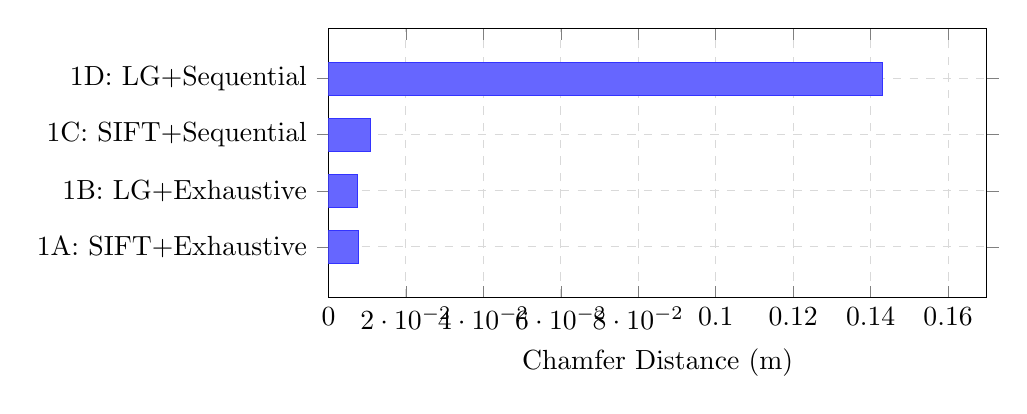
\begin{tikzpicture}
\begin{axis}[
    xbar, bar width=12pt,
    width=0.82\textwidth, height=5cm,
    symbolic y coords={1A,1B,1C,1D},
    ytick=data,
    yticklabels={
        {1A: SIFT+Exhaustive},
        {1B: LG+Exhaustive},
        {1C: SIFT+Sequential},
        {1D: LG+Sequential}},
    xlabel={Chamfer Distance (m)},
    xmin=0, xmax=0.17,
    enlarge y limits=0.3,
    grid=major, grid style={dashed,gray!30},
]
\addplot[fill=blue!60,draw=blue!80] coordinates {
    (0.007803,1A)(0.007437,1B)(0.010782,1C)(0.143084,1D)
};
\end{axis}
\end{tikzpicture}
\caption{Experiment 1 --- Chamfer Distance by matcher and strategy}
\label{fig:exp1_cd}
\end{figure}

\begin{figure}[H]
\centering
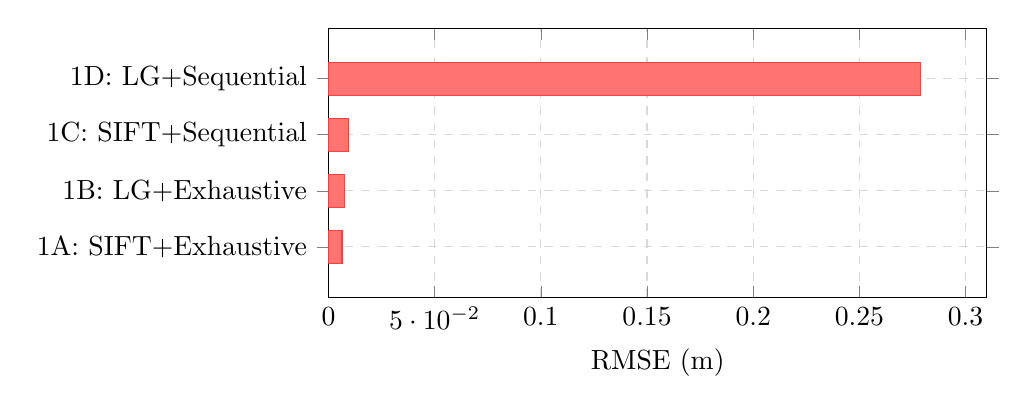
\begin{tikzpicture}
\begin{axis}[
    xbar, bar width=12pt,
    width=0.82\textwidth, height=5cm,
    symbolic y coords={1A,1B,1C,1D},
    ytick=data,
    yticklabels={
        {1A: SIFT+Exhaustive},
        {1B: LG+Exhaustive},
        {1C: SIFT+Sequential},
        {1D: LG+Sequential}},
    xlabel={RMSE (m)},
    xmin=0, xmax=0.31,
    enlarge y limits=0.3,
    grid=major, grid style={dashed,gray!30},
]
\addplot[fill=red!55,draw=red!75] coordinates {
    (0.006362,1A)(0.007368,1B)(0.009250,1C)(0.278657,1D)
};
\end{axis}
\end{tikzpicture}
\caption{Experiment 1 --- RMSE by matcher and strategy}
\label{fig:summary_en_exp1_rmse}
\end{figure}

\begin{multicols}{2}

\textbf{Experiment 2} identified a clear threshold effect for sequential overlap. Moving from overlap=5 to overlap=10 reduced Chamfer Distance by 0.033\,m; increasing beyond 10 yielded negligible further improvement. Overlap=10 was confirmed as the optimal setting for this dataset type.

\end{multicols}

% ── Experiment 2 chart ────────────────────────────────────────────────────
\begin{figure}[H]
\centering
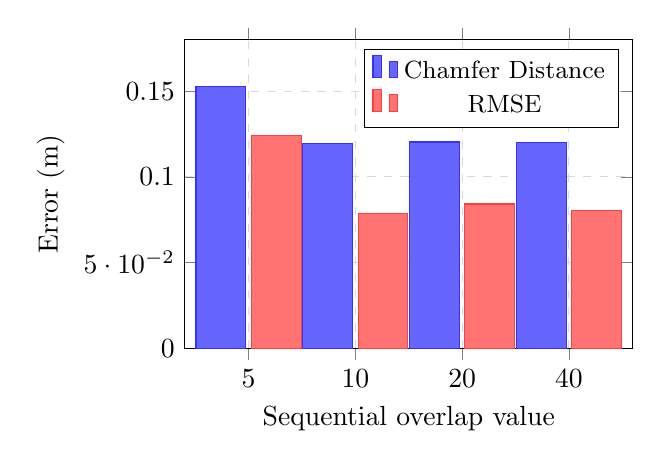
\begin{tikzpicture}
\begin{axis}[
    ybar, bar width=18pt,
    width=0.6\textwidth, height=5.5cm,
    symbolic x coords={5,10,20,40},
    xtick=data,
    xlabel={Sequential overlap value},
    ylabel={Error (m)},
    ymin=0, ymax=0.18,
    enlarge x limits=0.2,
    legend style={at={(0.97,0.97)},anchor=north east,font=\small},
    grid=major, grid style={dashed,gray!30},
]
\addplot[fill=blue!60,draw=blue!80] coordinates {
    (5,0.152750)(10,0.119549)(20,0.120356)(40,0.119830)
};
\addplot[fill=red!55,draw=red!75] coordinates {
    (5,0.123995)(10,0.078579)(20,0.084193)(40,0.080573)
};
\legend{Chamfer Distance, RMSE}
\end{axis}
\end{tikzpicture}
\caption{Experiment 2 --- Sequential overlap vs.\ error. Quality improves sharply from overlap=5 to overlap=10; gains beyond 10 are negligible.}
\label{fig:exp2}
\end{figure}

\begin{multicols}{2}

\textbf{Experiment 3} used the publicly available Lighthouse 4K video as a real-world outdoor input. A key methodological finding was that 3A's lower Chamfer Distance does not indicate superior reconstruction quality --- the 18$\times$ difference in reference point cloud size (952k vs.\ 17.5M points for 3B) makes direct cross-configuration comparison unreliable. Among the comparable configurations 3B and 3C, denser frame sampling reduced Chamfer Distance by 0.012\,m.

\end{multicols}

% ── Experiment 3 charts ───────────────────────────────────────────────────
\begin{figure}[H]
\centering
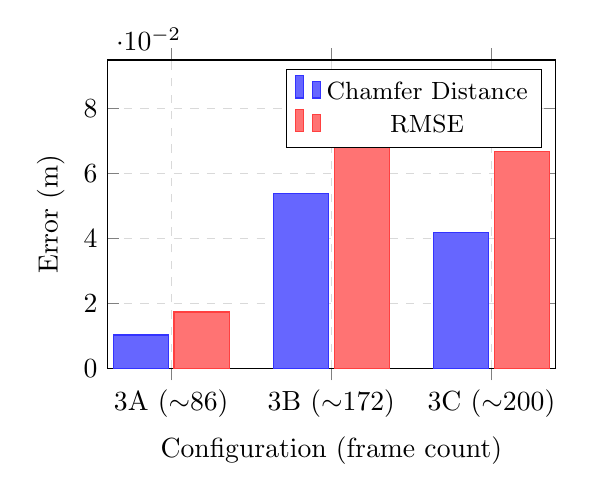
\begin{tikzpicture}
\begin{axis}[
    ybar, bar width=20pt,
    width=0.6\textwidth, height=5.5cm,
    symbolic x coords={3A (${\sim}$86),3B (${\sim}$172),3C (${\sim}$200)},
    xtick=data,
    xlabel={Configuration (frame count)},
    ylabel={Error (m)},
    ymin=0, ymax=0.095,
    enlarge x limits=0.2,
    legend style={at={(0.97,0.97)},anchor=north east,font=\small},
    grid=major, grid style={dashed,gray!30},
]
\addplot[fill=blue!60,draw=blue!80] coordinates {
    (3A (${\sim}$86),0.010333)
    (3B (${\sim}$172),0.053916)
    (3C (${\sim}$200),0.041948)
};
\addplot[fill=red!55,draw=red!75] coordinates {
    (3A (${\sim}$86),0.017397)
    (3B (${\sim}$172),0.082545)
    (3C (${\sim}$200),0.066822)
};
\legend{Chamfer Distance, RMSE}
\end{axis}
\end{tikzpicture}
\caption{Experiment 3 --- Frame sampling vs.\ error (Lighthouse 4K video). 3A is not directly comparable to 3B/3C due to an 18$\times$ difference in reference point cloud size.}
\label{fig:exp3_errors}
\end{figure}

\begin{figure}[H]
\centering
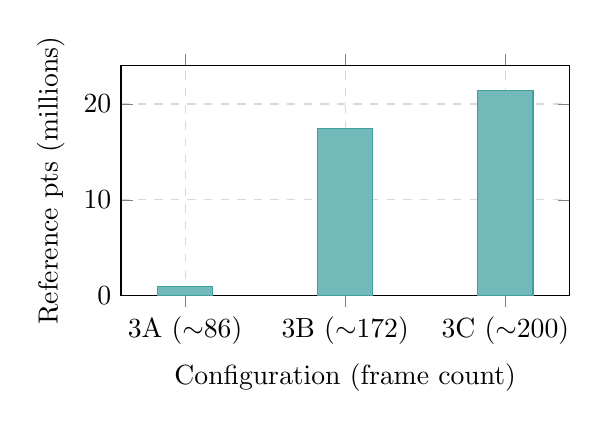
\begin{tikzpicture}
\begin{axis}[
    ybar, bar width=20pt,
    width=0.6\textwidth, height=4.5cm,
    symbolic x coords={3A (${\sim}$86),3B (${\sim}$172),3C (${\sim}$200)},
    xtick=data,
    xlabel={Configuration (frame count)},
    ylabel={Reference pts (millions)},
    ymin=0, ymax=24,
    enlarge x limits=0.2,
    grid=major, grid style={dashed,gray!30},
]
\addplot[fill=teal!55,draw=teal!75] coordinates {
    (3A (${\sim}$86),0.952)
    (3B (${\sim}$172),17.468)
    (3C (${\sim}$200),21.452)
};
\end{axis}
\end{tikzpicture}
\caption{Experiment 3 --- Reference point cloud size. The 18$\times$ gap between 3A and 3B/3C invalidates direct metric comparisons between them.}
\label{fig:exp3_pts}
\end{figure}

\begin{multicols}{2}

The following limitations are noted:
\begin{itemize}
    \item Only a single object type was tested (Exp.\ 1 \& 2); generalizability is unconfirmed,
    \item Unequal reference point cloud sizes in Exp.\ 3 make cross-configuration comparison unreliable,
    \item The GUI lacks a camera calibration interface,
    \item Sequential matching fails for certain matchers on small datasets.
\end{itemize}

From an engineering perspective, this work integrates the full reconstruction pipeline into a single cohesive PyQt5 GUI system. Future work includes integrating SuperPoint/SuperGlue and LightGlue under controlled conditions, comparing with NeRF and Gaussian Splatting, and extending evaluation to diverse object categories.

\noindent\textbf{5. References}

\small
\begin{enumerate}
    \item Hartley, R., \& Zisserman, A. (2003). \textit{Multiple View Geometry in Computer Vision}. Cambridge University Press.
    \item Lowe, D. G. (2004). Distinctive image features from scale-invariant keypoints. \textit{IJCV}, 60(2), 91--110.
    \item Sch{\"o}nberger, J. L., \& Frahm, J. M. (2016). Structure-from-motion revisited. \textit{CVPR}, 4104--4113.
    \item Cernea, D. (2015). OpenMVS: Multi-View Stereo Reconstruction Library.
    \item Mildenhall, B., et al. (2020). NeRF: Representing scenes as neural radiance fields. \textit{ECCV}, 405--421.
    \item Lindenberger, P., et al. (2023). LightGlue: Local feature matching at light speed. \textit{ICCV}, 17627--17638.
\end{enumerate}
\normalsize

\end{multicols}